% !Mode:: "TeX:UTF-8"
%%%%%%%%%%%%%%%%%%%%%%%%%%%%%%%%%%%%%%%%%%%%%%%%%%%%%%%%%%%%%%%%%%%%%%%%%%%%%%%%
%          ,
%      /\^/`\
%     | \/   |                CONGRATULATIONS!
%     | |    |             SPRING IS IN THE AIR!
%     \ \    /                                                _ _
%      '\\//'                                               _{ ' }_
%        ||                     hithesis v3                { `.!.` }
%        ||                                                ',_/Y\_,'
%        ||  ,                   dustincys                   {_,_}
%    |\  ||  |\          Email: yanshuoc@gmail.com             |
%    | | ||  | |            https://yanshuo.site             (\|  /)
%    | | || / /                                               \| //
%    \ \||/ /       https://github.com/dustincys/hithesis      |//
%      `\\//`   \\   \./    \\ /     //    \\./   \\   //   \\ |/ /
%     ^^^^^^^^^^^^^^^^^^^^^^^^^^^^^^^^^^^^^^^^^^^^^^^^^^^^^^^^^^^^^^
%%%%%%%%%%%%%%%%%%%%%%%%%%%%%%%%%%%%%%%%%%%%%%%%%%%%%%%%%%%%%%%%%%%%%%%%%%%%%%%%
\documentclass[fontset=fandol,toc=true,type=bachelor,stage=midterm,campus=harbin,toc=false]{hithesisart}
% 此处选项中不要有空格
%%%%%%%%%%%%%%%%%%%%%%%%%%%%%%%%%%%%%%%%%%%%%%%%%%%%%%%%%%%%%%%%%%%%%%%%%%%%%%%%
% 必填选项
% type=doctor|master|bachelor
% stage=opening|midterm
%%%%%%%%%%%%%%%%%%%%%%%%%%%%%%%%%%%%%%%%%%%%%%%%%%%%%%%%%%%%%%%%%%%%%%%%%%%%%%%%
% 选填选项(选填选项的缺省值已经尽可能满足了大多数需求,除非明确知道自己有什么
% 需求)
% campus=shenzhen|weihai|harbin
%   含义:校区选项,默认harbin
% fontset=windows|mac|ubuntu|fandol
%   含义:前三个对应各自系统,fandol是开源字体。
% toc=true|false
%   含义:是否显示目录,默认true
% newtxmath=true|false
%    含义:是否使用 times 风格数学字体,默认true
% print=true|false
%   含义:是否在封面后增加一个空白页用于打印,默认false
%%%%%%%%%%%%%%%%%%%%%%%%%%%%%%%%%%%%%%%%%%%%%%%%%%%%%%%%%%%%%%%%%%%%%%%%%%%%%%%%

\usepackage{float}
\graphicspath{{figures/}}


\begin{document}

% !Mode:: "TeX:UTF-8"

\hitsetup{
  %******************************
  % 注意:
  %   1. 配置里面不要出现空行
  %   2. 不需要的配置信息可以删除
  %******************************
  ctitlecover={载脂蛋白A1等蛋白质在\\ 国产处理器上的分子动力学模拟},%放在封面中使用,自由断行
  % ctitleone={局部多孔质气体静压},
  % ctitletwo={轴承关键技术的研究},
  caffil={化工与化学学院},
  csubject={应用化学},
  cauthor={龙英池},
  cstudentid={120L041204},
  cclassid={7203610828},
  csupervisor={杜耘辰教授},
  % 日期自动使用当前时间,若需指定按如下方式修改:
  %cdate={盘古开天地}
  % cenrolldate={公元2020年}
}

\makecover

% 深圳博士开题报告 -----------------------------------------------

% \input{body/report_shenzhen_doctor_opening}

% 威海校区本科生开题报告结构 ----------------------------------------
% \input{body/report_weihai_bachelor_opening}
% \makebackcover
% -------------------------------------------------------------

% 威海校区本科生中期报告结构 ----------------------------------------
% \input{body/report_weihai_bachelor_midterm}
% \makebackcover
% -------------------------------------------------------------

% 哈尔滨校区本科生开题报告结构 --------------------------------------
\section{课题来源及研究的目的和意义}

载脂蛋白A1 (ApoA1) 为附着于高密度脂蛋白(HDL)及乳靡小球上的载脂蛋白。
是构成血浆中高密度脂蛋白(HDL)蛋白质部分的主要成分。
ApoA1 在体内脂质代谢的角色相当重要,因此常被视为预测个体冠心病风险的生物标记。
ApoA1 在癌症诊断\cite{limwjxtd}、预后预测\cite{apoayuhz}等方面有重要作用。
因此,利用分子动力学方法,模拟 ApoA1 的构象变化、折叠过程,对于生物医学、化学等研究有重要意义。


\begin{figure}[h]
    \centering
    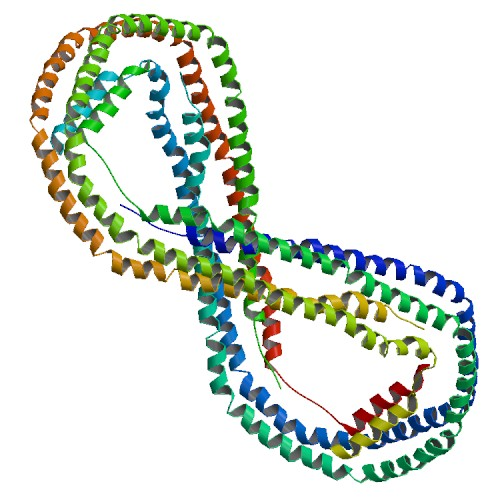
\includegraphics[width=0.4\textwidth]{images/PBB_Protein_APOA1_image.jpg}
    \caption{ApoA1 在蛋白质数据库 (PDB) 中的渲染结果}
\end{figure}

计算科学与高性能计算在当代科学研究和工程应用中扮演着至关重要的角色。
分子动力学模拟作为一种重要的计算科学工具,广泛用于模拟分子体系的行为,如生物分子、聚合物和复合材料。
其中,NAMD(NAnoscale Molecular Dynamics)\cite{phillips2005scalable}是一款广泛应用的分子动力学软件,其高度并行的特性使其成为模拟大规模分子系统的有力工具。
然而,目前,NAMD在国产CPU上的性能与一些国际竞争对手相比存在一定差距。


\begin{figure}[h]
    \centering
    
\includegraphics{images/namd-logo.png}
    \caption{NAMD 标识}
\end{figure}

本项目计划从 ApoA1 等蛋白质出发,在国产 CPU 上完成对这些蛋白质的分子动力学模拟计算,为国内科研和工程应用提供更高效的分子动力学模拟解决方案。
通过优化NAMD算法,我们将探讨如何充分利用国产CPU的硬件资源,提高模拟速度,降低计算成本,并使国内科研机构和工程部门能够更好地应对复杂的分子系统建模问题。

研究的意义在于不仅促进了分子动力学模拟的发展,还有助于推动国产CPU技术在科学计算领域的应用和发展。
这项研究将有助于提高我国在生物医药、材料科学、化学工程等领域的研究和创新水平,为国家自主研发计算机技术提供实际应用的范例。
最终,通过这项研究,我们将为国内高性能计算和科学研究社区提供一种有效的分子模拟工具,为我国的科学研究和工程应用带来巨大的潜在价值。

\section{国内外在该方向的研究现状及分析}

\subsection{载脂蛋白 A1 的研究}

载脂蛋白A1 是一种重要的蛋白质,参与高密度脂蛋白(HDL)颗粒的形成和维护,对体内胆固醇代谢和心血管健康至关重要。
2023 年,李媚和她的同事报道了载脂蛋白在HBV相关肝癌诊断中的价值\cite{limwjxtd}。
同年,李子胜团队研究了载脂蛋白对系统性红斑狼疮活动性和预后不良预测价值\cite{apoayuhz}。

\subsection{分子动力学计算与 NAMD 软件}

分子动力学在化学、医学方向的应用十分广泛。
其基本原理是对广义牛顿运动方程的求解。

分子动力学模拟要求按一定的时间步长对经典运动方程进行不连续的积分,而时间步长受制于分子体系中运动最快的自由度。 在对势加和的方法中,理论上的计算开销复杂度为 $O(n^2)$,即体系中粒子数的平方。
在实际计算中,对静电相互作用中的短程力部分可采用球形截断策略,而求解Poisson方程时则可采用离散化的处理方案,这样,就可以在倒易空间(reciprocal space)里处理长程相互作用,从而使实际的计算开销减少到$O(n\log n)$。

20世纪80年代末,为了能更高效地处理超大生物体系的计算,人们对串行分子动力学代码相应地进行了并行化,同时致力于开发更适合于硬件前沿技术的全新计算策略。在当时诸多开创性的工作中,值得一提的是Heller等\cite{heller1990molecular}开发的第一个可扩展的分子动力程序EGO。
EGO是现代并行分子动力学程序的先驱,可在大型集群上并行运行。
EGO利用多步长积分算法和自适应快速多偶极算法处理长程静电相互作用,从而在40000个原子的范围内能够使复杂度优化到 $O(n)$ (即,与原子数大致成线性关系)。

随着并行化体系结构的发展和计算规模的提升,人们发现仅仅使用 OpenMP 等优化方法编写并行程序是不够用的。人们开始重新编写程序来应对高度并行的超级计算机系统。
其中,随着空间分配算法\cite{brown1993domain}的提出,一批高度并行化的分子动力学计算软件相继问世,
例如,NAMD\cite{phillips2005scalable}, AMBER\cite{case2008amber}, GROMACS\cite{abraham2015gromacs}, LAMMPS\cite{thompson2022lammps}等。

表 \ref{tab:md-comparison} 列出了这些软件的优缺点。

\begin{table}[h]
    \centering
    \caption{分子动力学软件比较}
    \label{tab:md-comparison}
    \begin{tabular}{ccc}
        \toprule
        名称      & 优点                       & 缺点        \\
        \midrule
        NAMD    & 设计水平高、计算效率高              & 不适合多糖体系模拟 \\
        AMBER   & 有很好的内置势能模型               & 计算效率不高    \\
        LAMMPS  & 兼任目前大多数势能模型,效率优(不如 NAMD) & 维护差       \\
        GROMACS & 算法优秀,计算效率高,维护好           & 势能模型兼容性不好 \\
        \bottomrule
    \end{tabular}
\end{table}

NAMD 是一种开源高性能分子动力学模拟软件,用于模拟原子和分子之间的相互作用以及它们的运动行为。
NAMD的主要应用领域包括生物医学研究\cite{yao2020molecular}、生物化学\cite{knott2020characterization}、药物设计\cite{han2020computational}、材料科学和纳米技术。
这个软件的独特之处在于其能够模拟极小尺度的系统,如生物分子、蛋白质、DNA、聚合物和其他化学体系,以揭示它们的结构、动力学和相互作用。

% 国外,超算上的应用
% 2020 Gorden Bell 用了这个软件
2020年 Lorenzo Casalino 等人利用 NAMD 模拟了 SARS-CoV-2 病毒 (俗称新冠病毒)的刺突蛋白(图 \ref{fig:sars-cov-2-spike})的动力学过程\cite{casalino2021ai},展示了 NAMD 在大规模计算上的作用。

\begin{figure}[h]
    \centering
    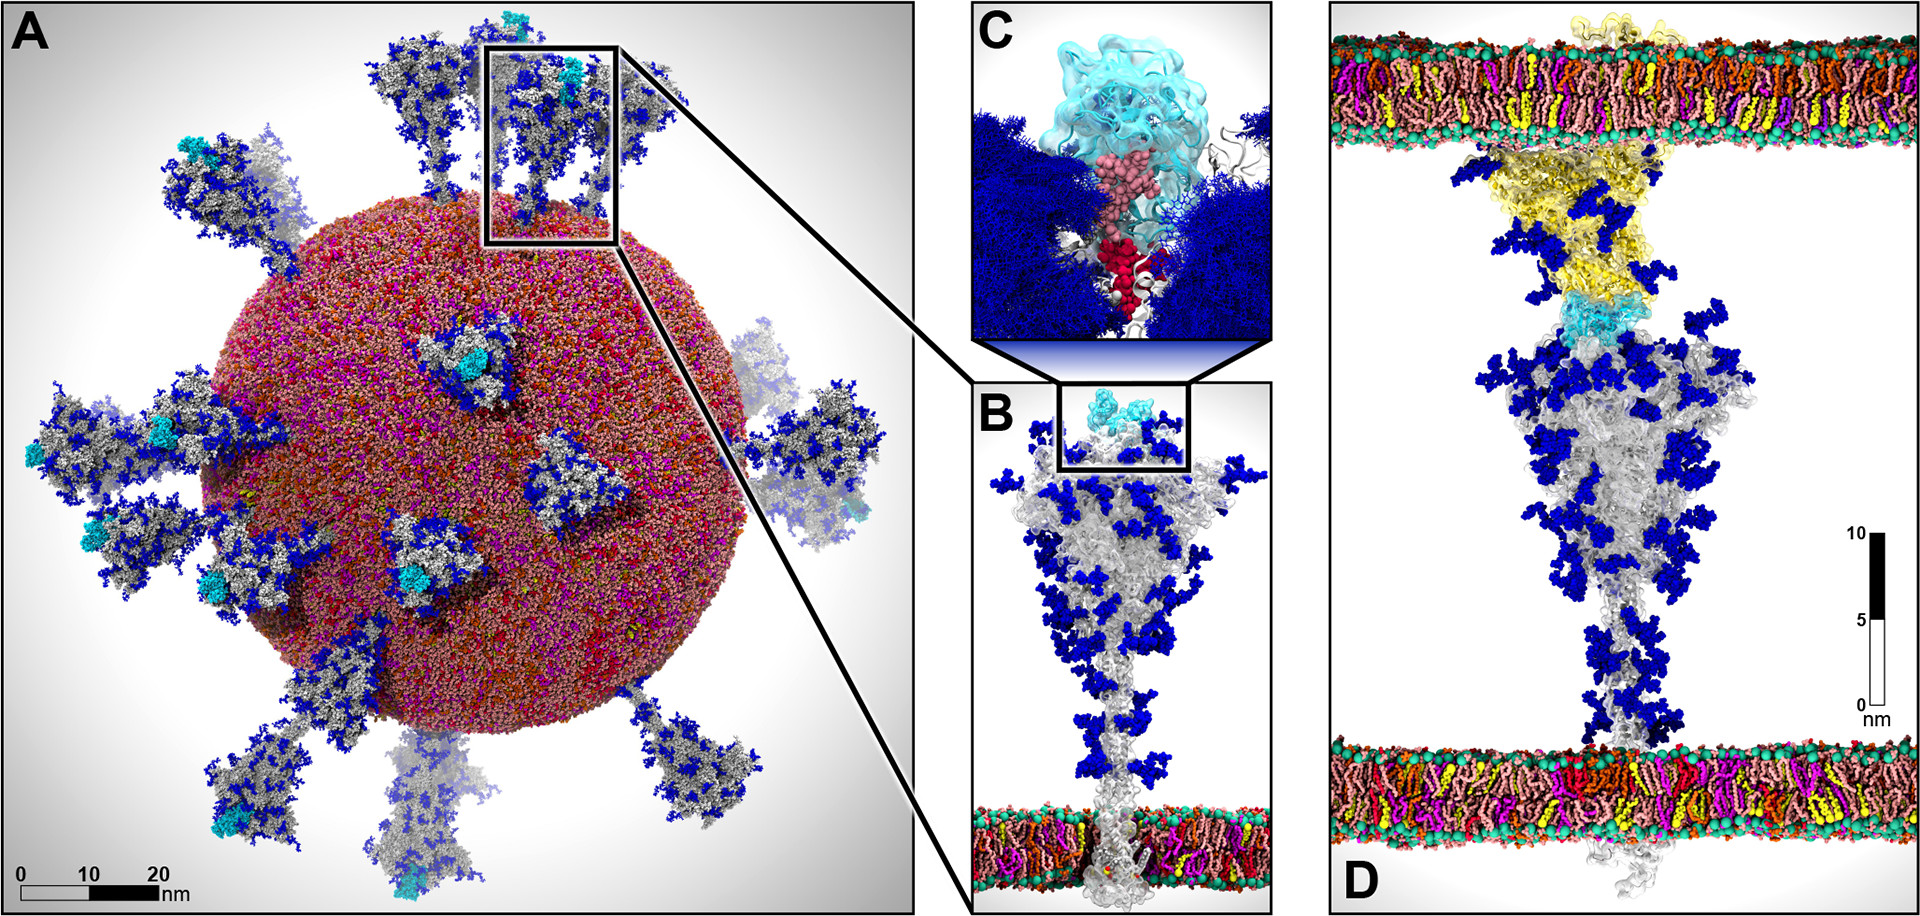
\includegraphics[width=0.6\textwidth]{images/spike.jpeg}
    \caption{SARS-CoV-2 的刺突蛋白}
    \label{fig:sars-cov-2-spike}
\end{figure}

% 国内
2010年,刘倩等人在中国科学院网络与信息中心深腾7000平台测试了 NAMD 的性能,并对STMV典型的烟草花叶卫星病毒进行了2048处理器核的模拟计算\cite{刘倩2010基于深腾}。
深腾计算机采取了采用混合架构的高性能计算集群,由 Intel Xeon 处理器集群与 Intel Itanium2 胖节点组成,主要采用的是 Intel 公司的 x86 指令集架构。
2017年,姚文军\cite{姚文军2017基于神威太湖之光的}等人将 NAMD 移植到了神威太湖之光上。

\section{主要研究内容}

本项目计划从 ApoA1 等蛋白质出发,在国产 CPU 上完成对这些蛋白质的分子动力学模拟计算。主要研究内容包括:

\subsection{蛋白质结构分析}

NAMD 主要用于蛋白质体系的分子动力学计算。
在计算前,需要获取蛋白质的基本结构数据,包括原子的数量和位置、环境参数等参数。
另外,还需要获取蛋白质原子之间的成键情况。

\subsection{了解分子动力学计算基本原理}

另外,还需要充分了解分子动力学计算的基本原理,包括分子的运动规律、相互作用势函数的概念,以及系综的选择方法。

势函数描述了分子之间的相互作用,涵盖了静电相互作用、范德华力、键角弯曲力等各种相互作用力,这些力在计算中起着关键作用,决定了分子在模拟中的行为。

此外,也需要深入了解系综的选择方法,因为不同的物理系统和问题需要不同类型的系综,如NVE系综、NVT系综或NPT系综等,以适应不同的温度、压力和能量约束条件。
系综的选择方法对于模拟结果的可靠性和适用性至关重要,因此在进行分子动力学模拟前,必须明确选择适当的系综以满足研究需求。

\subsection{自主指令集架构了解与适应}

研究团队需要深入了解国产自主指令集架构,包括其体系结构特点、指令集编程模型和硬件特性。
这将有助于更好地理解如何将 NAMD 移植到该架构上,并为后续的优化工作奠定基础。

\subsection{NAMD 移植工作}

将 NAMD 软件移植到国产自主指令集架构上,确保其在该架构上的基本运行。这包括适应指令集、调整编译工具链以支持目标架构,并解决与体系结构相关的兼容性问题。

\subsection{性能评估与基准测试}


在这一阶段,研究小组计划对移植后的 NAMD 进行详细的性能评估测试,这有助于深入了解它在自主指令集架构上的性能表现。这一细致的评估过程将涵盖多个方面,其中之一是进行广泛的基准测试和性能分析,以精确地量化其性能,并进一步比较其与现有架构的性能差距。

在基准测试方面,我们将选取载脂蛋白 A1 (ApoA1) 等分子体系作为评估体系,包括大蛋白质复合物、脂质双层膜或水合离子作为测试样例,评估移植后的 NAMD 在处理不同系统和场景下的性能。
通过在这些多样性的测试案例中进行性能比较,我们可以更全面地了解 NAMD 在自主指令集架构上的性能表现。

性能分析也将涵盖多个方面,包括计算速度、内存使用、能源效率等。我们将监测在不同硬件平台上的 NAMD 运行时间,以及它在利用 SIMD 指令扩展时的效率提升。此外,我们还将关注内存占用情况,以确保 NAMD 在自主指令集架构上的性能改进不伴随显著的内存负担。最后,能源效率的评估将考虑在高性能计算集群中的 NAMD 运行所需的能源消耗,以便更全面地评估其可持续性和经济性。

通过这些详尽的性能评估和基准测试,我们将能够全面了解移植后的 NAMD 在自主指令集架构上的性能表现,从而为未来的分子动力学模拟研究和应用提供有力的支持和指导。

\section{研究方案}

\section{目前已完成的研究工作及结果}

项目已经对 NAMD 软件在 Intel 平台上进行了蛋白质模拟计算,并且在国产 CPU 上完成了 NAMD 的初步移植工作,可以计算出一些小分子物质的极化率、势能、动能等数据。

\subsection{调研蛋白质的性质与规模,收集蛋白质空间数据}

蛋白质的原子数目是影响分子动力学计算负载的关键。
载脂蛋白 A1 含有 92224 个原子,在经典蛋白质体系中原子数较少。
其他一些蛋白质体系的原子数目在表 \ref{tab:protein-size} 中列出。

\begin{table}[h]
    \centering
    \caption{一些蛋白质、大分子体系的原子数规模}
    \label{tab:protein-size}
    \begin{tabular}{ccc}
        \toprule
        名称       & 简写     & 原子数目    \\
        \midrule
        载脂蛋白 A1  & ApoA1  & 92224   \\
        ATP合成酶   & ATPASE & 327506  \\
        卫星烟草花叶病毒 & STMV   & 1066628 \\
        \bottomrule
    \end{tabular}
\end{table}

除了蛋白质的性质规模外,还需研究蛋白质的三维结构数据。

蛋白质数据库(Protein Data Bank,简称PDB)\cite{burley2017protein,sussman1998protein} 是一个专门收录蛋白质及核酸的三维结构资料的数据库。

可以从蛋白质数据库中下载所需要的蛋白质的原子位置信息,以及初始速度,格式为 PDB 文件。
另外,还需要蛋白质原子之间的成键信息,这些成键信息在 PSF 中储存。

表 \ref{tab:protein-files} 中列出了这两种信息文件。

\begin{table}[h]
    \centering
    \caption{从蛋白质数据库中下载的蛋白质信息文件}
    \label{tab:protein-files}
    \begin{tabular}{cc}
        \toprule
        格式  & 文件包含的信息  \\
        \midrule
        PDB & 原子位置、速度  \\
        PSF & 原子之间成键情况 \\
        \bottomrule
    \end{tabular}
\end{table}

目前,已经下载到了丙氨酸、ApoA1、STMV 等蛋白质的 PDB 文件和 PSF 文件。他们可以被加载到 VMD 中,观察蛋白质的三维结构。



\subsection{分子动力学计算}

分子动力学计算的基本原理是对广义牛顿运动方程的求解。
系统的总势能为系统中各个原子的位置的函数 $U = (\vec{r_1}, \vec{r_2}, \dots, \vec{r_N})$。
在系统中的任意原子 $i$ ,根据牛顿力学,其受理和势函数关系为


\begin{equation}
    \vec{F} = -\nabla U (\vec{r_1}, \vec{r_2}, \dots, \vec{r_N}) = - \left( \vec{i} \frac{\partial}{\partial x_x} + \vec{j}\frac{\partial}{\partial x_y} + \vec{k} \frac{\partial}{\partial x_z}\right) U
\end{equation}

系统内任意原子的加速度和受力关系为\cite{易浩杰2019纳米静电喷射的分子动力学模拟研究}

\begin{equation}
    a_i = \frac{F_i}{m_i} = \frac{\mathrm{d}^2 r}{\mathrm{d} t^2}
\end{equation}

\subsection{计算结果、含义}

NAMD 的输入、输出均为 PDB 蛋白质数据库文件,用以描述分子每次迭代的位置和速度。
分子动力学软件基于牛顿力学计算每个原子在力场下的运动情况,迭代若干次按时间计算每个原子的位置和速度,因此输出的计算结果主要是\textit{位置} (.coor) 和\textit{速度} (.vel) 两个文件。

这些输出文件对于研究者来说具有深远的意义。位置文件(.coor)提供了分子中每个原子在空间中的具体坐标,这对于了解分子的结构、构象变化以及相互作用至关重要。另一方面,速度文件(.vel)则展示了每个原子的瞬时运动状态,这对于分析分子的动力学行为、温度效应等方面具有重要价值。

另外,如果需要计算分子的热力学性质,如极化率、内能,自由能,则包含更多计算量。


\subsection{各个蛋白质计算结果}

\subsubsection{HIV-1 蛋白酶复合物 (PDB 1a30) 的配体,49原子}

\begin{figure}[h]
    \centering
    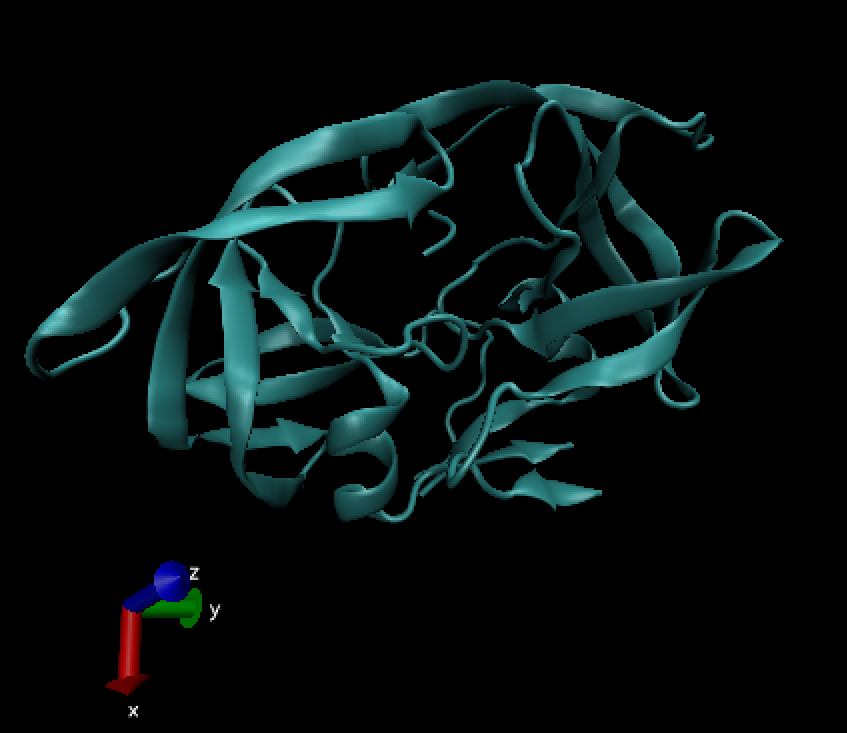
\includegraphics[width=0.5\textwidth]{images/1A30.png}
    \caption{HIV-1 蛋白酶复合物 (PDB 1a30) 的配体, VMD}
    \label{fig:1a30}
\end{figure}


PDB 1a30 蛋白质是 HIV-1 (人类免疫缺陷病毒)蛋白酶复合物的配体(图 \ref{fig:1a30} ),我们在曙光集群上用两个节点迭代62次,计算其极化性( $ 10^{-3} \cdot C/m^2$ )。


\begin{equation}
    \alpha = \begin{bmatrix}
        285.0 & -16.6 & 4.2   \\
        -16.6 & 245.3 & 20.5  \\
        4.2   & 20.5  & 271.2 \\
    \end{bmatrix}
\end{equation}


\subsubsection{丙氨酸 (66原子)}

\begin{figure}[h]
    \centering
    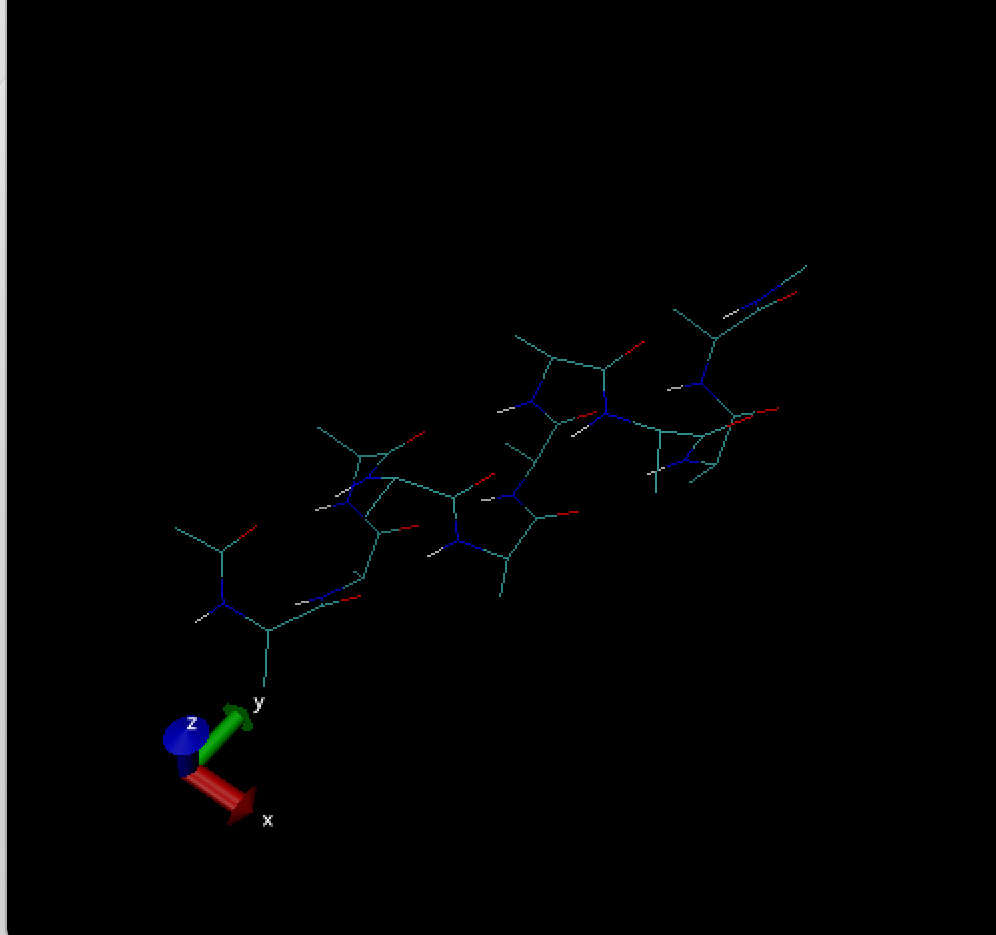
\includegraphics[width=0.5\textwidth]{images/alanin.png}
    \caption{丙氨酸 (66原子)}
    \label{fig:alanin}
\end{figure}

\subsubsection{载脂蛋白A1 (92224原子)}

2023 年 11 月,软件成功在神威上模拟了载脂蛋白 A1 的运动情况,如图 \ref{fig:apoa1} 所示。

\begin{figure}[h]
    \centering
    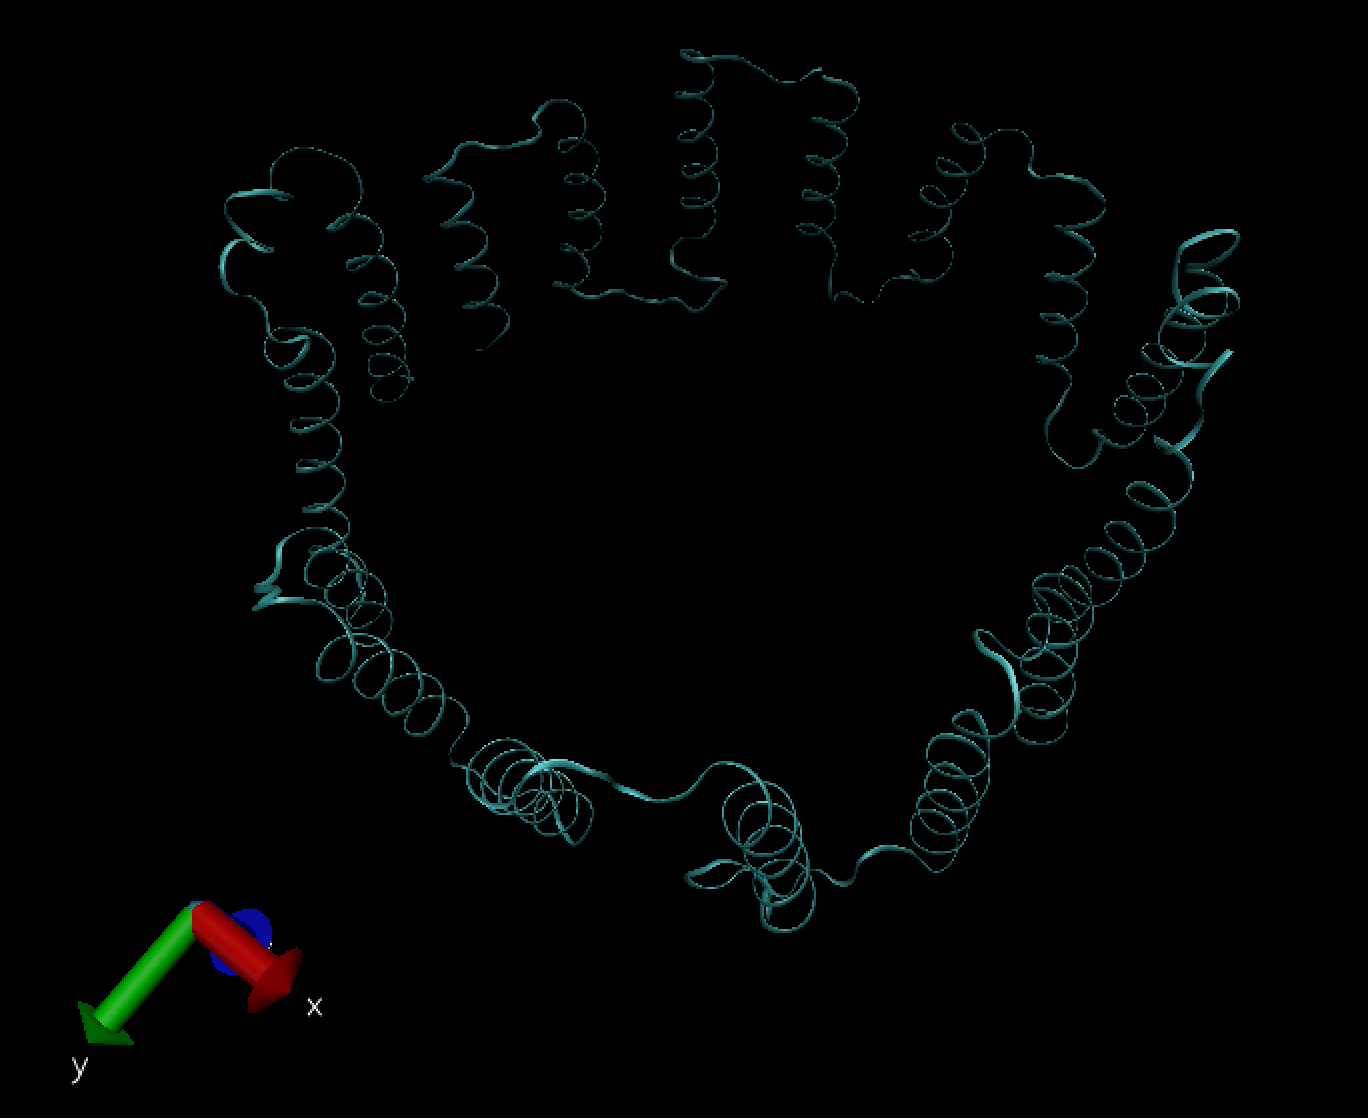
\includegraphics[width=0.5\textwidth]{images/ApoA1.png}
    \caption{载脂蛋白A1 (92224原子)}
    \label{fig:apoa1}
\end{figure}

图 \ref{fig:apoa1-plot} 展示了载脂蛋白 A1 的 500 步分子动力学模拟,每一步分子总动能和势能的变化趋势。
而在这500步模拟中,图 \ref{fig:apoa1-plot} 中可以看出,载脂蛋白 A1 在水溶液中动能、势能的相互转换趋势,以及在溶液体系中能量的耗散情况。
动力学模拟呈现了载脂蛋白 A1在分子水平上的动态特征,为我们提供了深入了解其结构和运动的视角。

\begin{figure}[h]
    \centering
    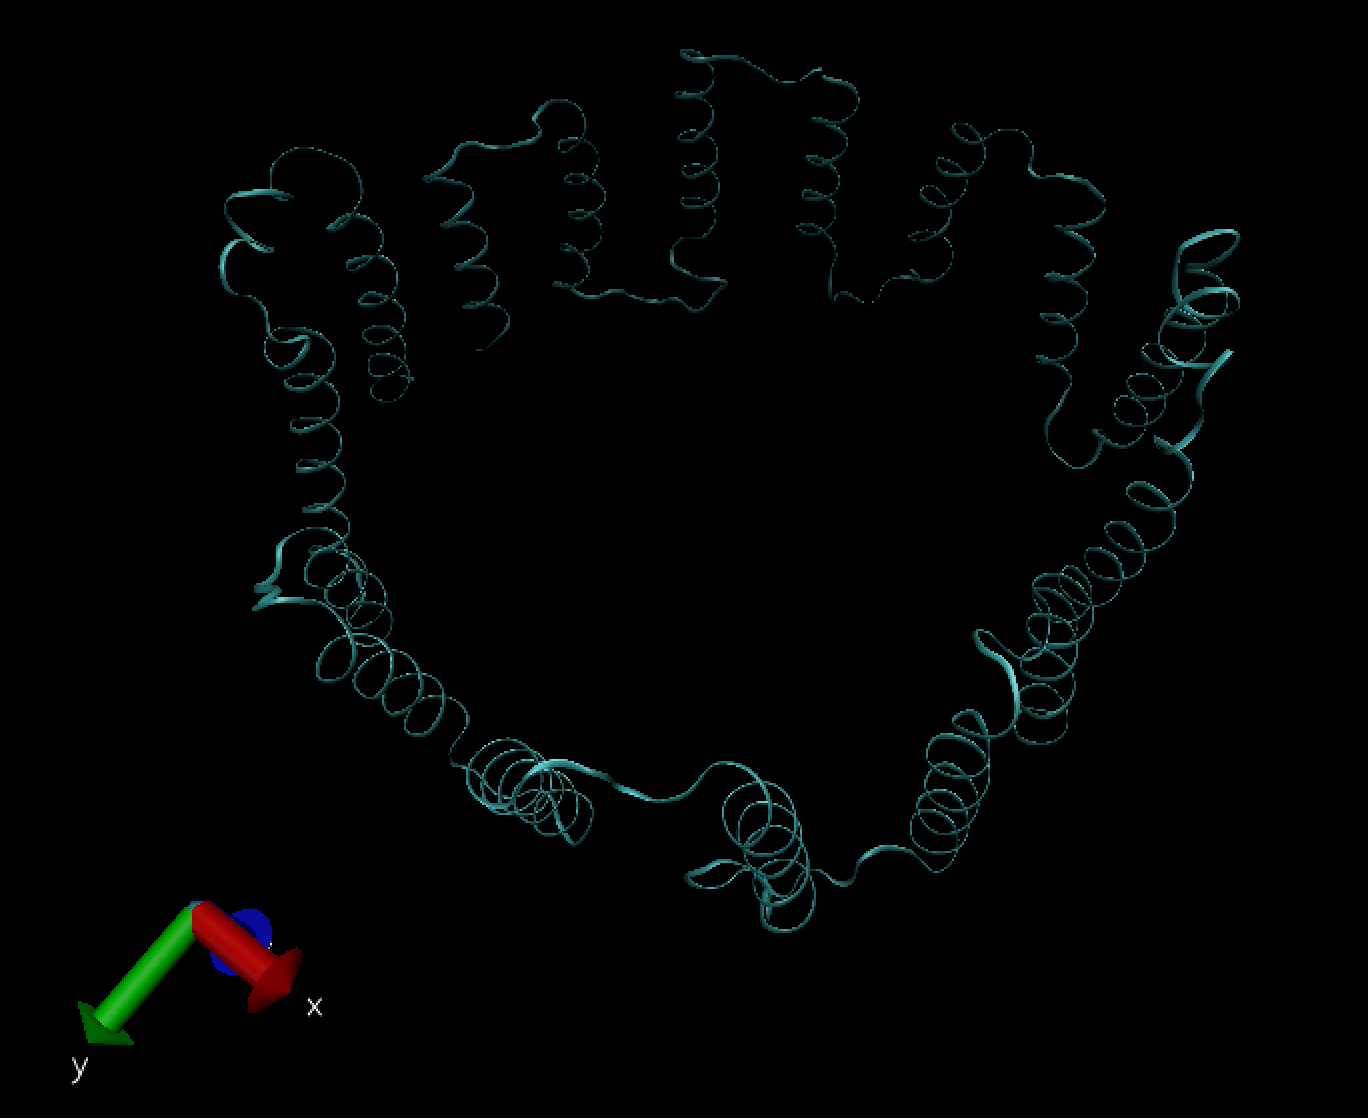
\includegraphics[width=0.7\textwidth]{images/ApoA1.pdf}
    \caption{载脂蛋白 A1 500步模拟,能量变化趋势(动能、势能)}
    \label{fig:apoa1-plot}
\end{figure}


\subsubsection{STMV (virus, 1066628 原子)}

\begin{figure}[h]
    \centering
    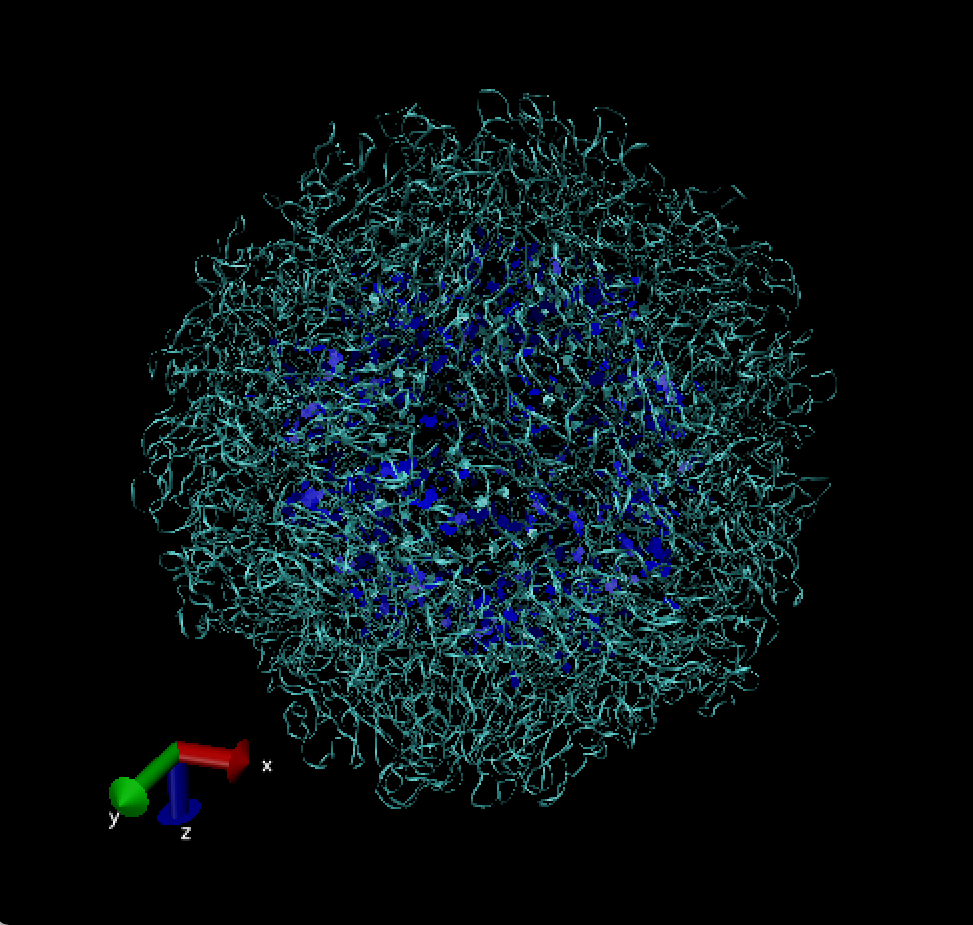
\includegraphics[width=0.5\textwidth]{images/STMV.png}
    \caption{STMV (virus, 1066628 原子)}
    \label{fig:stmv}
\end{figure}

\begin{figure}[h]
    \centering
    \includegraphics[width=0.9\textwidth]{images/stmv.pdf}
    \caption{卫星烟草花叶病毒 (STMV) 500步模拟,能量变化趋势(动能、势能)}
    \label{fig:stmv-plot}
\end{figure}

卫星烟草花叶病毒是一种二十面体的植物病毒,这种病毒会加重烟草花叶病毒感染症状。
卫星烟草花叶病毒是自然界中最小的,可自我复制的单位,它不仅依赖花叶细胞,也依赖被感染的烟草花叶病毒。
卫星烟草花叶病毒共包含 1066628 原子,为中等规模的蛋白质测试用例。
图 \ref{fig:stmv} 展示了卫星烟草花叶病毒的可视化外观。
图 \ref{fig:stmv-plot} 则展示了卫星烟草花叶病毒 500 步动力学模拟的能量变化趋势。




\section{存在的困难与问题}



\subsection{优化方案分析}

本项目计划采用单指令流多数据流 (Single Instruction Multiple Data, SIMD) 指令扩展来提高分子动力学模拟性能。
图 \ref{fig:simd} 展示了 SIMD 在处理器上的设计,它可以提供多个数据供一条指令使用,从而并行执行多个算术运算,提升性能。


首先,我们将针对现有的分子动力学模拟软件进行必要的修改,以支持 SIMD 指令扩展。
这将涉及到重写现有的 NAMD 计算内核,以便能够同时处理多个数据元素。

分子动力学模拟中出现最多的计算量有力、位置、能量,这些都是三维的量。
因此为了使用 SIMD 需要补充一个维度,这会涉及到一些代价估计计算工作。


\begin{figure}[h]
    \centering
    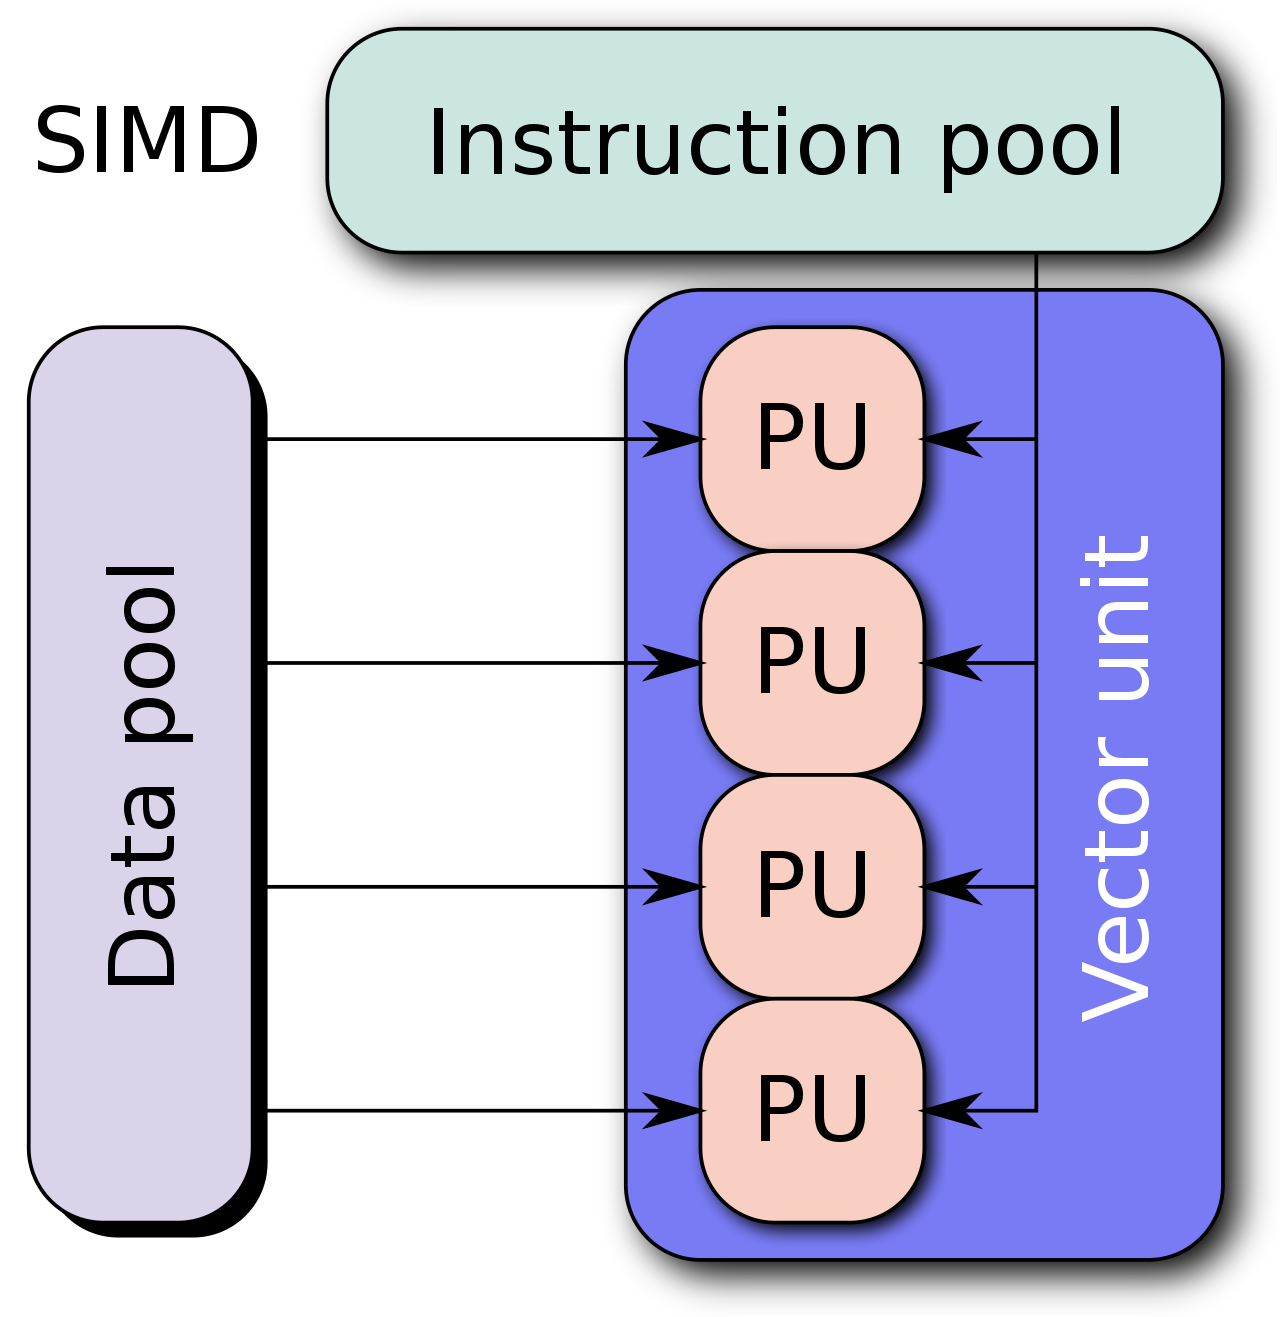
\includegraphics[width=0.3\textwidth]{images/SIMD2.svg.png}
    \caption{SIMD 在体系结构上的设计图示}
    \label{fig:simd}
\end{figure}

\section{进度安排,预期达到的目标}

\subsection{进度安排}

表 \ref{tab:progress} 展示了本项目的进度安排表。我们将从立项时间 $T_1$ 开始逐步完成每个任务。

\section{后期拟完成的研究工作及进度安排}

在中期报告中,我已成功完成了将NAMD软件移植到专用处理器上的任务,为分子动力学模拟提供了加速的可能性。接下来的研究工作将着重于优化和进一步提升模拟的效率,以满足高性能计算的需求。以下是后期拟完成的研究工作及进度安排:

\begin{enumerate}
    \item \textbf{性能优化}: 针对专用处理器的特性,对NAMD进行性能优化,包括但不限于利用处理器的并行性、矢量化指令等,以最大程度地发挥硬件加速的潜力。
    \item \textbf{并行计算}:进一步优化并行计算策略,充分利用专用处理器的多核心架构,实现更高效的计算并提高模拟的整体吞吐量。
    \item \textbf{性能评估与调优}:对移植后的NAMD进行详细的性能评估,识别潜在的瓶颈和性能瓶颈,并进行进一步的调优工作,以达到最佳的性能表现。
    \item \textbf{应用案例研究}:在一系列分子动力学模拟案例中验证优化后的NAMD在专用处理器上的性能。通过模拟复杂分子系统,评估加速效果和模拟质量。
\end{enumerate}


\begin{table}[h]
    \centering
    \caption{进度安排表}
    \label{tab:progress}
    \begin{tabular}{cc}
        \toprule
        时间 (立项时间为 $T_1$) & 进度                              \\
        \midrule
        $T_1$ + 1 月      & 蛋白质数据库收集与了解                     \\
        $T_1$ + 3 月      & NAMD 在 Intel CPU 上的蛋白质计算模拟      \\
        $T_1$ + 6 月      & NAMD 在 国产 CPU 上的初步移植与正确性验证 中期检查 \\
        $T_1$ + 9 月      & 蛋白质在国产 CPU 上的模拟和优化              \\
        $T_1$ + 12 月     & 项目结题                            \\
        \bottomrule
    \end{tabular}
\end{table}



\section{主要参考文献}
\bibliographystyle{hithesis}
\bibliography{reference}

% Local Variables:
% TeX-master: "../mainart"
% TeX-engine: xetex
% End:

% -------------------------------------------------------------

\end{document}

% Local Variables:
% TeX-engine: xetex
% End:
